\vspace*{1em}

\begin{discussion}
Let $A,B$ be sets, recall that a function
\[f: A \to B\]
is a ``rule'' that assigns an element of $B$ to every element of $A$. We note the following.
\begin{itemize}
\item[(i)] $\dom(f) = A$. ($f$ is defined for every element of $A$)
\item[(ii)] For each $a \in A$, $f$ assigns a \emph{unique} element $f(a) \in B$.
\end{itemize}
We now give a formal definition of a function $f:A \to B$ in terms of relations.
\end{discussion}

\vspace*{1em}

\begin{definition}
Let $A,B$ be non-empty sets. A \cdef{function} {\color{blue}$f:A \to B$} is a relation $f \subseteq A \times B$ from $A$ to $B$ such that for every $a \in A$
\[\text{if $afb$ and $afc$, then $b = c$;}\]
or equivalently we have  \[\abs{f \cap (\set{a} \times B)} = 1\] i.e. for every $a \in A$, there is a single element in $f$ with $a$ as the first coordinate.\\
\\
That is, for every $a \in A$, there is a unique $b \in B$ that is $f$-related to $a$; that is, for every $a$, there is a unique $b$ such that $(a,b) \in f$. In this case, we write $b = f(a)$. Notationally, we have
\begin{align*}
f: A &\to B\\
 a&\mapsto b
\end{align*}
With the $a \mapsto b$ notation meaning $b = f(a)$.\\
\\
With this notation, a relation $f$ is a function if for any $a,c \in A$,
\[a = c \text{ implies } f(a) = f(c)\]
Verifying this property to show that a given relation is a function is called \emph{showing $f$ is well-defined}.\\
\\
As a relation, $f$ has a domain and range. We have $\dom(f) = A$ and $\range(f) = \setp{f(a)}{a \in A}$. To note, the range can be a proper subset of $B$; we call $B$ the \cdef{codomain} of $f$, we denote $\mathrm{codom}(f) = B$.

\vspace*{0.5em}

\begin{remark}
In terms of our notation, the function $f$ as a relation, that is, as a subset of $A \times B$, is
\[f = \setp{(a,f(a))}{a \in A} \subseteq A \times B,\]
which is what we usually call the \emph{graph of $f$}.
\end{remark}
\end{definition}

\vspace*{1em}

\begin{example}[some abstract examples]\hfill
\begin{itemize}
\item[$\bullet$] \emph{Identity function}.\\[0.5em]
For any set $X$, the \emph{identity function on $X$} is the function
\begin{align*}
\id_X: X &\to X\\
 x&\mapsto x
\end{align*}
That is, this is the function $\id_X(x) = x$. As a relation, this is just the diagonal subset
\[\id_X = \setp{(x,x)}{x \in X} \subseteq X \times X\]

\item[$\bullet$] \emph{Inclusion function}.\\[0.5em]
For any non-empty set $A$, and a subset $C \subseteq A$. The inclusion function is the function
\begin{align*}
\iota : C &\to A\\
 c&\mapsto c
\end{align*}
As a relation, this is the subset
\[\iota = \setp{(c,c)}{c \in C} \subseteq C \times A\]

\item[$\bullet$] \emph{Restriction function}.\\[0.5em]
Let $f:A \to B$ be a function, and consider a subset $C \subseteq A$. Then, the relation
\[f\vert_C \defeq f \cap (C \times B)\]
is a function. This is now a function 
\begin{align*}
f\vert_C : C &\to B\\
 c&\mapsto f(c)
\end{align*}
where $\dom(f\vert_C) = C$. That is, given the rule $f$ on $A$, we are restricting this rule to a subset.
\end{itemize}
\end{example}

\vspace*{1em}

\begin{definition}
Let $f: A \to B$ be a function, and let $C \subseteq A$ and $D \subseteq B$.
\begin{itemize}
\item[$\bullet$] The \cdef{image\ of} {\color{blue}$C$} \cdef{under} {\color{blue}$f$} is the set 
\[f(C) \defeq \setp{f(x)}{x \in C} \subseteq B\]
Note that $\range(f) = f(A)$.
\[\begin{tikzpicture}[scale=0.9]
\draw[thick] (0,0) ellipse (1.25cm and 2.5cm);
\filldraw[pattern=crosshatch dots, thick] (0,0) ellipse (0.75cm and 1.5cm);

\draw[thick] (4,0) ellipse (1cm and 2cm);
\filldraw[fill=newblue, fill opacity=1/2, thick] (4,0) ellipse (0.5cm and 1cm);

\draw[thick,dashed] (0,1.5) -- (4,1);
\draw[thick,dashed] (0,-1.5) -- (4,-1);
\draw[->,thick] (1.5,0) -- (2.75,0) node[midway,above] {$f$};

\node[above] at (0,2.5) {$A$};
\node[above] at (4,2) {$B$};

\node[below] at (0,-1.5) {\small$C$};
\node[below] at (4,-1) {\small$f(C)$};
\end{tikzpicture}\]
\item[$\bullet$] The \cdef{preimage\ of} {\color{blue}$D$} \cdef{under} {\color{blue}$f$} is the set 
\[f^{-1}(D) \defeq \setp{y \in A}{f(y) \in D} \subseteq A\]
\[\begin{tikzpicture}[scale=0.9]
\draw[thick] (0,0) ellipse (1.5cm and 2.35cm);
\filldraw[fill=firebrick, fill opacity=1/2, thick] (0,0) ellipse (0.6cm and 1.2cm);

\draw[thick] (4,0) ellipse (1cm and 2cm);
\filldraw[pattern=crosshatch dots, thick] (4,0) ellipse (0.45cm and 0.9cm);

\draw[thick,dashed] (0,1.2) -- (4,0.9);
\draw[thick,dashed] (0,-1.2) -- (4,-0.9);
\draw[->,thick] (1.75,0) -- (2.75,0) node[midway,above] {$f$};

\node[above] at (0,2.35) {$A$};
\node[above] at (4,2) {$B$};

\node[below] at (0,-1.2) {\small$f^{-1}(D)$};
\node[below] at (4,-0.9) {\small$D$};
\end{tikzpicture}\]
\end{itemize}

\end{definition}

\vspace*{1em}

\begin{definition}
Let $A,B$ be non-empty sets. Define,
\[B^A = \setp{f:A \to B}{\text{$f$ is a function}}\]
\end{definition}

\vspace*{1em}

\begin{lemma}
For non-empty finite sets $A,B$, we have $|B^A| = \abs{B}^{\abs{A}}$.
\end{lemma}
\begin{proof}
Each element in $A$ has $\abs{B}$-many choices to be mapped to. Each such choice gives us a unique function. Since each element has $\abs{B}$-many choices, the total number of functions from $A$ to $B$ is
\[\underbrace{\abs{B} \cdot \abs{B} \cdots \abs{B}}_{\abs{A} \text{-times}} = \abs{B}^{\abs{A}}\]
This completes the proof. 
\end{proof}

\vspace*{1em}

\begin{definition}
Let $f:A \to B$  be a function.
\begin{itemize}
\item[$\bullet$] $f$ is said to be \cdef{injective} (or {\color{blue}\cdef{one}-\cdef{to}-\cdef{one}}) if ``$f$ maps distinct elements to distinct elements''; that is, if for every $x,y \in A,\ x \neq y$ implies $f(x) \neq f(y)$.
\[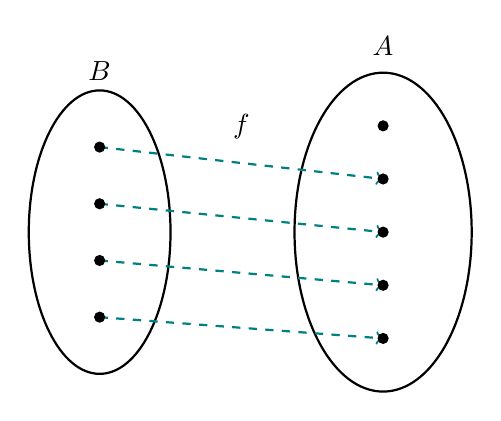
\begin{tikzpicture}[scale=0.9]
\draw[thick] (0,0) ellipse (1cm and 2cm);
\draw[thick] (4,0) ellipse (1.25cm and 2.25cm);

\draw[->,thick,dashed,teal] (0,1.2) -- (4,0.75) node[midway,above,yshift=5pt] {\color{black}$f$};
\draw[->,thick,dashed,teal] (0,0.4) -- (4,0);
\draw[->,thick,dashed,teal] (0,-0.4) -- (4,-0.75);
\draw[->,thick,dashed,teal] (0,-1.2) -- (4,-1.5);

\filldraw (0,1.2) circle (2pt);
\filldraw (0,0.4) circle (2pt);
\filldraw (0,-0.4) circle (2pt);
\filldraw (0,-1.2) circle (2pt);

\filldraw (4,1.5) circle (2pt);
\filldraw (4,0.75) circle (2pt);
\filldraw (4,0) circle (2pt);
\filldraw (4,-0.75) circle (2pt);
\filldraw (4,-1.5) circle (2pt);

\node[above] at (4,2.35) {$A$};
\node[above] at (0,2) {$B$};
\end{tikzpicture}\]
Equivalently, taking the contrapositive, $f$ is \cdef{injective} if for every $x,y \in A,\ f(x) = f(y)$ implies $x = y$. This definition is more convenient for proofs.\\
\\
$B$ has a ``copy of $A$ inside it''.

\item[$\bullet$] $f$ is said to be \cdef{surjective} (or \cdef{onto}) if $f(A) = B$.
\[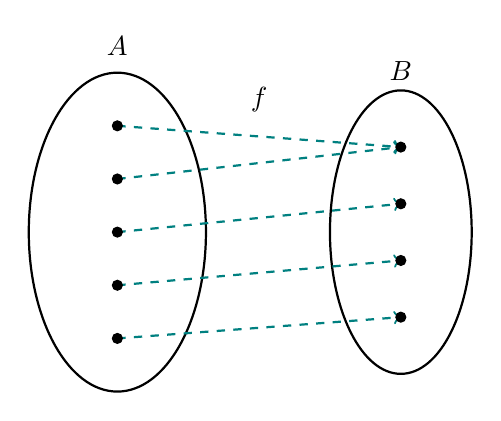
\begin{tikzpicture}[scale=0.9]
\draw[thick] (4,0) ellipse (1cm and 2cm);
\draw[thick] (0,0) ellipse (1.25cm and 2.25cm);

\draw[->,thick,dashed,teal] (0,1.5) -- (4,1.2) node[midway,above,yshift=5pt] {\color{black}$f$};
\draw[->,thick,dashed,teal] (0,0.75) -- (4,1.2);
\draw[->,thick,dashed,teal] (0,0) -- (4,0.4);
\draw[->,thick,dashed,teal] (0,-0.75) -- (4,-0.4);
\draw[->,thick,dashed,teal] (0,-1.5) -- (4,-1.2);

\filldraw (4,1.2) circle (2pt);
\filldraw (4,0.4) circle (2pt);
\filldraw (4,-0.4) circle (2pt);
\filldraw (4,-1.2) circle (2pt);

\filldraw (0,1.5) circle (2pt);
\filldraw (0,0.75) circle (2pt);
\filldraw (0,0) circle (2pt);
\filldraw (0,-0.75) circle (2pt);
\filldraw (0,-1.5) circle (2pt);

\node[above] at (0,2.35) {$A$};
\node[above] at (4,2) {$B$};
\end{tikzpicture}\]
Equivalently, ``if every element in $B$ is mapped to by $f$'', that is, for every $b \in B$, there exists an $a \in A$ such that $b = f(a)$ (this is just saying $B \subseteq f(A)$).%\\
%\\
%The set $A$ is ``partially collapsed'', in the sense that several elements of $A$ map to the same element of $B$, and all elements of $B$ are obtained in this way.

\item[$\bullet$] $f$ is \cdef{bijective} if it is both injective and surjective.
\[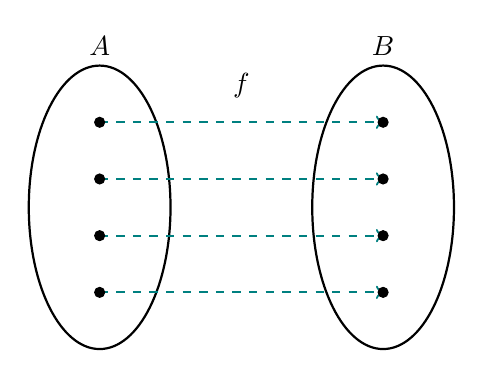
\begin{tikzpicture}[scale=0.9]
\draw[thick] (4,0) ellipse (1cm and 2cm);
\draw[thick] (0,0) ellipse (1cm and 2cm);

\draw[->,thick,dashed,teal] (0,1.2) -- (4,1.2) node[midway,above,yshift=5pt] {\color{black}$f$};
\draw[->,thick,dashed,teal] (0,0.4) -- (4,0.4);
\draw[->,thick,dashed,teal] (0,-0.4) -- (4,-0.4);
\draw[->,thick,dashed,teal] (0,-1.2) -- (4,-1.2);

\filldraw (4,1.2) circle (2pt);
\filldraw (4,0.4) circle (2pt);
\filldraw (4,-0.4) circle (2pt);
\filldraw (4,-1.2) circle (2pt);

\filldraw (0,1.2) circle (2pt);
\filldraw (0,0.4) circle (2pt);
\filldraw (0,-0.4) circle (2pt);
\filldraw (0,-1.2) circle (2pt);

\node[above] at (0,2) {$A$};
\node[above] at (4,2) {$B$};
\end{tikzpicture}\]
$f$ gives an exact correspondence of elements between $A$ and $B$. So sets $A$ and $B$ have the ``same size''. 
\end{itemize}
\end{definition}

\vspace*{1em}

\begin{example}
A function $f: \rr\setminus\set{2} \to \rr\setminus\set{3}$ is given by 
\[f(x) = 3 + \frac{6}{x - 2}\]
($f$ is not defined for $x = 2$ and its value can never be $3$).\\[0.5em]
Show that $f$ is a bijection.
\end{example}
\begin{proof}
We show $f$ is injective and bijective. To show $f$ is injective, suppose $x,y \neq 2$ are such that $f(x) = f(y)$, we want to show $x = y$. So, note
\begin{align*}
f(x) &= f(y)\\[0.5em]
3 + \frac{6}{x - 2} &= 3 + \frac{6}{y - 2}\\[0.5em]
\frac{6}{x - 2} &= \frac{6}{y - 2} &&& \text{subtracting $3$}\\[0.5em]
6(y - 2) &= 6(x - 2) &&& \text{cross-multiplying}\\[0.5em]
6y - 12 &= 6x - 12\\[0.5em]
\end{align*}
\begin{align*}
6y &= 6x &&& \text{adding $12$}\\[0.5em]
y &= x &&& \text{dividing by $6$}
\end{align*}
Thu, $f$ is injective.\\
\\
To show $f$ is surjective, let $b \in \rr\setminus\set{3}$. We show that there exists an element $a \in \rr\setminus\set{2}$ such that $f(a) = b$.\\

\begin{subproof}
\begin{proof}[Scratch work]\renewcommand{\qed}{}
We will work backwards to find such an $a$; suppose we did have $f(a) = b$, we solve for $a$.
\begin{align*}
3 + \frac{6}{a - 2} &= f(a) = b\\[0.5em]
\frac{6}{a - 2} &= b - 3 &&& \text{subtracting $3$}\\[0.5em]
\frac{a - 2}{6} &= \frac{1}{b - 3} &&& \text{taking reciprocal, we can since $b \neq 3$}\\[0.5em]
a - 2 &= \frac{6}{b - 3} &&& \text{multiplying by $6$}\\[0.5em]
a &= 2 + \frac{6}{b - 3} &&& \text{adding $2$}
\end{align*}
Note that this expression is $\neq 2$.
\end{proof}
\end{subproof}
\vspace*{0.5em}
For given $b$, consider
\[a = 2 + \frac{6}{b - 3} \in \rr\setminus\set{2}\]
This is such that 
\begin{align*}
f(a) &= 3 + \frac{6}{a - 2}\\[1em]
 &= 3 + \frac{6}{\left(2 + \frac{6}{b - 3}\right) - 2}\\[1em]
 &= 3 + \frac{6}{\frac{6}{b - 3}}\\[1em]
 &= 3 + \frac{6(b-3)}{6}\\[1em]
 &= 3 + (b-3)\\[0.5em]
 &= b
\end{align*}
Thus $f$ is surjective.\\
\\
This completes the proof. 
\end{proof}

\vspace*{1em}

\begin{discussion}
We can characterise injectivity and surjectivity in another way. Let $f:A \to B$ be a function. For any $b \in B$, we can consider its pre-image
\[f^{-1}(\set{b}) = \setp{a \in A}{f(a) = b}\]
$f$ is injective if and only if $|f^{-1}(\set{b})| \leq 1$ for every $b \in B$.\\[0.5em]
$f$ is surjective if and only if $|f^{-1}(\set{b})| \geq 1$ for every $b \in B$.\\[0.5em]
Therefore $f$ is bijective if and only if $|f^{-1}(\set{b})| = 1$.
\end{discussion}

\vspace*{1em}

\begin{definition}[Composition of Functions]
Let $f:A \to B$ and $g:B \to C$ be functions. Then their \cdef{composition} is the function
\[g\circ f: A \to C\]
defined as \[(g\circ f)(a) = g(f(a))\] for any $a \in A$.
\end{definition}

\vspace*{1em}

\begin{proposition}
Let $f:A \to B$ and $g:B \to C$ be functions.
\begin{itemize}
\item[(1)] If both $f$ and $g$ are injective, then their composition $g \circ f$ is also injective. 
\item[(2)] If both $f$ and $g$ are surjective, then their composition $g \circ f$ is also surjective. 
\end{itemize}
\end{proposition}
\[\begin{tikzpicture}[scale=0.65]
\draw[thick] (9,0) ellipse (1.8cm and 3.6cm);
\draw[thick] (4,0) ellipse (1.4cm and 2.8cm);
\draw[thick] (0,0) ellipse (1cm and 2cm);

\draw[->,thick,dashed,newblue] (0,1.2) -- (4,1.2) node[midway,above,yshift=5pt] {\color{black}$f$};
\draw[->,thick,dashed,newblue] (0,0.4) -- (4,0.4);
\draw[->,thick,dashed,newblue] (0,-0.4) -- (4,-0.4);
\draw[->,thick,dashed,newblue] (0,-1.2) -- (4,-1.2);

\draw[->,thick,dashed,firebrick] (4,2) -- (9,2) node[midway,above,yshift=5pt] {\color{black}$g$};
\draw[->,thick,dashed,firebrick] (4,1.2) -- (9,1.2);
\draw[->,thick,dashed,firebrick] (4,0.4) -- (9,0.4);
\draw[->,thick,dashed,firebrick] (4,-0.4) -- (9,-0.4);
\draw[->,thick,dashed,firebrick] (4,-1.2) -- (9,-1.2);
\draw[->,thick,dashed,firebrick] (4,-2) -- (9,-2);

\filldraw (9,2.8) circle (2pt);
\filldraw (9,2) circle (2pt);
\filldraw (9,1.2) circle (2pt);
\filldraw (9,0.4) circle (2pt);
\filldraw (9,-0.4) circle (2pt);
\filldraw (9,-1.2) circle (2pt);
\filldraw (9,-2) circle (2pt);
\filldraw (9,-2.8) circle (2pt);

\filldraw (4,2) circle (2pt);
\filldraw (4,1.2) circle (2pt);
\filldraw (4,0.4) circle (2pt);
\filldraw (4,-0.4) circle (2pt);
\filldraw (4,-1.2) circle (2pt);
\filldraw (4,-2) circle (2pt);

\filldraw (0,1.2) circle (2pt);
\filldraw (0,0.4) circle (2pt);
\filldraw (0,-0.4) circle (2pt);
\filldraw (0,-1.2) circle (2pt);

\node[above] at (0,2) {$A$};
\node[above] at (4,2.8) {$B$};
\node[above] at (9,3.6) {$C$};
\end{tikzpicture}\]
\begin{proof}[Proof of (1)]
Suppose $f$ and $g$ are injective, we need to show $g\circ f$ is injective. Consider any $x, y \in A$ such that $(g\circ f)(x) = (g\circ f)(y)$, we need to show $x = y$. We have,
\[g(f(x)) = g(f(y)),\]
since $g$ is injective, we have $f(x) = f(y)$. Now, since $f$ is injective, we obtain $x = y$.  Hence $g\circ f$ is injective.
\end{proof}
\[\begin{tikzpicture}[scale=0.65]
\draw[thick] (0,0) ellipse (1.8cm and 3.6cm);
\draw[thick] (5,0) ellipse (1.4cm and 2.8cm);
\draw[thick] (9,0) ellipse (1cm and 2cm);

\draw[->,thick,dashed,newblue] (0,2.8) -- (5,2) node[midway,above,yshift=5pt] {\color{black}$f$};
\draw[->,thick,dashed,newblue] (0,2) -- (5,2);
\draw[->,thick,dashed,newblue] (0,1.2) -- (5,1.2);
\draw[->,thick,dashed,newblue] (0,0.4) -- (5,0.4);
\draw[->,thick,dashed,newblue] (0,-0.4) -- (5,-0.4);
\draw[->,thick,dashed,newblue] (0,-1.2) -- (5,-0.4);
\draw[->,thick,dashed,newblue] (0,-2) -- (5,-1.2);
\draw[->,thick,dashed,newblue] (0,-2.8) -- (5,-2);

\draw[->,thick,dashed,firebrick] (5,2) -- (9,1.2) node[midway,above,yshift=5pt] {\color{black}$g$};
\draw[->,thick,dashed,firebrick] (5,1.2) -- (9,0.4);
\draw[->,thick,dashed,firebrick] (5,0.4) -- (9,0.4);
\draw[->,thick,dashed,firebrick] (5,-0.4) -- (9,-0.4);
\draw[->,thick,dashed,firebrick] (5,-1.2) -- (9,-0.4);
\draw[->,thick,dashed,firebrick] (5,-2) -- (9,-1.2);

\filldraw (0,2.8) circle (2pt);
\filldraw (0,2) circle (2pt);
\filldraw (0,1.2) circle (2pt);
\filldraw (0,0.4) circle (2pt);
\filldraw (0,-0.4) circle (2pt);
\filldraw (0,-1.2) circle (2pt);
\filldraw (0,-2) circle (2pt);
\filldraw (0,-2.8) circle (2pt);

\filldraw (5,2) circle (2pt);
\filldraw (5,1.2) circle (2pt);
\filldraw (5,0.4) circle (2pt);
\filldraw (5,-0.4) circle (2pt);
\filldraw (5,-1.2) circle (2pt);
\filldraw (5,-2) circle (2pt);

\filldraw (9,1.2) circle (2pt);
\filldraw (9,0.4) circle (2pt);
\filldraw (9,-0.4) circle (2pt);
\filldraw (9,-1.2) circle (2pt);

\node[above] at (9,2) {$C$};
\node[above] at (5,2.8) {$B$};
\node[above] at (0,3.6) {$A$};
\end{tikzpicture}\]
\begin{proof}[Proof of (2)]
Suppose $f$ and $g$ are surjective, we need to show $g\circ f$ is surjective. We aim to show that for every $c \in C$, we can find an $a \in A$ such that $(g\circ f)(a) = c$.\\[0.5em]
Consider any $c \in C$, since $g$ is surjective, there exists a $b \in B$ such that $g(b) = c$. Since $f$ is surjective, for this $b$, there exists an $a \in A$ such that $f(a) = b$. Hence, \[(g\circ f)(a) = g(f(a)) = g(b) = c.\] Thus $g\circ f$ is surjective. 
\end{proof}

\vspace*{1em}

What about the converse?
\begin{proposition}\label{thm:compinsur}
Let $f:A \to B$ and $g:B \to C$ be functions.
\begin{itemize}
\item[(1)] If $g \circ f$, then $f$ is injective. 
\[\begin{tikzpicture}[scale=0.8]
\draw[thick] (0,0) ellipse (1cm and 1.4cm);
\draw[thick] (4,0) ellipse (1cm and 2cm);
\draw[thick] (8,0) ellipse (1cm and 2cm);

\draw[->,thick,dashed,newblue] (0,0.8) -- (4,0.4) node[midway,above,yshift=5pt] {\color{black}$f$};
\draw[->,thick,dashed,newblue] (0,0) -- (4,-0.4);
\draw[->,thick,dashed,newblue] (0,-0.8) -- (4,-1.2);

\draw[->,thick,dashed,firebrick] (4,1.2) -- (8,0.4) node[midway,above,yshift=5pt] {\color{black}$g$};
\draw[->,thick,dashed,firebrick] (4,0.4) -- (8,0.4);
\draw[->,thick,dashed,firebrick] (4,-0.4) -- (8,-0.4);
\draw[->,thick,dashed,firebrick] (4,-1.2) -- (8,-1.2);

\filldraw (0,0.8) circle (2pt);
\filldraw (0,0) circle (2pt);
\filldraw (0,-0.8) circle (2pt);

\filldraw (4,1.2) circle (2pt);
\filldraw (4,0.4) circle (2pt);
\filldraw (4,-0.4) circle (2pt);
\filldraw (4,-1.2) circle (2pt);

\filldraw (8,1.2) circle (2pt);
\filldraw (8,0.4) circle (2pt);
\filldraw (8,-0.4) circle (2pt);
\filldraw (8,-1.2) circle (2pt);

\node[above] at (8,2) {$C$};
\node[above] at (4,2) {$B$};
\node[above] at (0,1.4) {$A$};
\end{tikzpicture}\]
\[\text{\emph{$g$ need not be injective in (1)}}\]
\item[(2)] If $g \circ f$ is surjective, then $g$ is surjective.
\[\begin{tikzpicture}[scale=0.8]
\draw[thick] (0,0) ellipse (1cm and 2cm);
\draw[thick] (4,0) ellipse (1cm and 2.35cm);
\draw[thick] (8,0) ellipse (1cm and 1.2cm);

\draw[->,thick,dashed,newblue] (0,1.2) -- (4,1.6) node[midway,above,yshift=5pt] {\color{black}$f$};
\draw[->,thick,dashed,newblue] (0,0.4) -- (4,1.6);
\draw[->,thick,dashed,newblue] (0,-0.4) -- (4,0);
\draw[->,thick,dashed,newblue] (0,-1.2) -- (4,-0.8);

\draw[->,thick,dashed,firebrick] (4,1.6) -- (8,0.4) node[midway,above,yshift=5pt] {\color{black}$g$};
\draw[->,thick,dashed,firebrick] (4,0.8) -- (8,0.4);
\draw[->,thick,dashed,firebrick] (4,0) -- (8,-0.4);
\draw[->,thick,dashed,firebrick] (4,-0.8) -- (8,-0.4);
\draw[->,thick,dashed,firebrick] (4,-1.6) -- (8,-0.4);

\filldraw (0,1.2) circle (2pt);
\filldraw (0,0.4) circle (2pt);
\filldraw (0,-0.4) circle (2pt);
\filldraw (0,-1.2) circle (2pt);

\filldraw (4,1.6) circle (2pt);
\filldraw (4,0.8) circle (2pt);
\filldraw (4,0) circle (2pt);
\filldraw (4,-0.8) circle (2pt);
\filldraw (4,-1.6) circle (2pt);

\filldraw (8,0.4) circle (2pt);
\filldraw (8,-0.4) circle (2pt);

\node[above] at (8,1.2) {$C$};
\node[above] at (4,2.35) {$B$};
\node[above] at (0,2) {$A$};
\end{tikzpicture}\]
\[\text{\emph{$f$ need not be surjective in (2)}}\]
\end{itemize}
\end{proposition}

\begin{proof}[Proof of (1)]
Suppose $g\circ f$ is injective, we need to show $f$ is injective. Consider any $x, y \in A$ such that $f(x) = f(y)$, we need to show $x = y$.\\[0.5em] 
Since $f(x) = f(y)$, therefore $g(f(x)) = g(f(y))$. That is,
\[g(f(x)) = g(f(y)).\]
Since $g\circ f$ is injective, we obtain $x = y$.  Hence $f$ is injective.
\end{proof}
\begin{proof}[Proof of (2)]
Suppose $g\circ f$ is surjective, we need to show $g$ is surjective. We aim to show that for every $c \in C$, we can find an $b \in B$ such that $g(b) = c$.\\[0.5em]
Consider any $c \in C$, since $g\circ f$ is surjective, there exists a $a \in A$ such that $(g\circ f)(a) = c$. Define $b = f(a)$, then $g(b) = g(f(a)) = (g\circ f)(a) = c$. Hence $g$ is surjective. 
\end{proof}

\vspace*{1em}

\begin{definition}
Two functions $f$ and $g$ are said to be equal, denoted $f = g$ if
\begin{itemize}
\item[(1)] $\dom f = \dom g$; and
\item[(2)] $f(x) = g(x)$ for every $x \in \dom f = \dom g$.
\end{itemize}
\end{definition}

\vspace*{1em}

\begin{theorem}
Let $f:A \to B$ and $g:B \to A$ be functions. Suppose,
\[g\circ f = \id_A \quad \text{and} \quad f\circ g = \id_B\]
Then $f$ and $g$ are bijective, and are inverses of each other as relations.\\[0.5em]
\emph{We call $g$ the \emph{inverse function} of $f$ (or vice versa)}.
\end{theorem}
\begin{remark}
Often the most convenient way to show a function $f:A \to B$ is bijective is to find a function $g:B \to A$ such that $f\circ g = \id_B$ and $g\circ f = \id_A$. If we can find such a function, we do not have give a separate argument on the injectivity and surjectivity of $f$. 
\end{remark}
\begin{proof}
Since the identity functions are bijective, we obtain that $g\circ f$ and $f\circ g$ are both bijective. In particular, $g\circ f$ and $f \circ g$ are injective, therefore by Theorem \ref{thm:compinsur} (1), we obtain $f$ and $g$ are injective respectively. We also have that $g\circ f$ and $f \circ g$ are surjective, therefore by Theorem \ref{thm:compinsur} (2), we obtain $f$ and $g$ are surjective. Hence, both $f$ and $g$ are injective and surjective, and thus bijective.\\
\\
Since $g\circ f = \id_A$, one can show by set inclusion arguments that as relations $g = f^{-1}$, where $f^{-1}$ is the inverse relation of $f$. That is, in this case the relation $f^{-1}$ is a function (in fact, $f^{-1}$ is a function if and only if $f$ is bijective).
\end{proof}

\vspace*{1em}

\begin{example}
A function $f: \rr\setminus\set{2} \to \rr\setminus\set{3}$ is given by 
\[f(x) = 3 + \frac{6}{x - 2}\]
Show that $f$ is a bijection.
\end{example}
\begin{proof}
We produce an inverse function to prove $f$ is bijective.\\
\begin{subproof}
\begin{proof}[Scratch work]\renewcommand{\qed}{}
We do some algebra to obtain the inverse function. 
\begin{itemize}[leftmargin=3.5em]
\item[Step 1.] First let $y = f(x)$, that is,
\[y = 3 + \frac{6}{x - 2}\]
\item[Step 2.] Replace $x$ by $y$ and vice versa. That is,
\[x = 3 + \frac{6}{y - 2}\]
\item[Step 3.] Solve for $y$.
\begin{align*}
3 + \frac{6}{y - 2} &= x\\[0.5em]
\frac{6}{y - 2} = x - 3 &&& \text{subtracting $3$}\\[0.5em]
\frac{y - 2}{6} = \frac{1}{x - 3} &&& \text{taking reciprocal, we can since $b \neq 3$}\\[0.5em]
y - 2 = \frac{6}{x - 3} &&& \text{multiplying by $6$}\\[0.5em]
y = 2 + \frac{6}{x - 3} &&& \text{adding $2$}
\end{align*}
Note that this expression is $\neq 2$.
\item[Step 4.] The resulting $y$ is your candidate for an inverse function.
\end{itemize}
\end{proof}
\end{subproof}
\vspace*{0.5em}
Define $g: \rr\setminus\set{3} \to \rr\setminus\set{2}$ as
\[g(x) = 2 + \frac{6}{x - 3}\]
Then,
\begin{align*}
(g\circ f)(x) = g(f(x)) &= 2 + \frac{6}{f(x) - 3} & (f\circ g)(x) = f(g(x)) &= 3 + \frac{6}{g(x) - 2}\\[1em]
 &= 2 + \frac{6}{\left(3 + \dfrac{6}{x - 2}\right) - 3} & &= 3 + \frac{6}{\left(2 + \dfrac{6}{x - 3}\right) - 2}\\[1em]
 &= 2 + \frac{6}{\left(\dfrac{6}{x - 2}\right)} & &= 3 + \frac{6}{\left(\dfrac{6}{x - 3}\right)}\\[1em]
 &= 2 + \frac{6(x-2)}{6} & &= 3 + \frac{6(x-3)}{6}\\[1em]
 &= 2 + (x - 2) = x & &= 3 + (x - 3)  = x
\end{align*}
Hence $f\circ g = \id$ and $g\circ f = \id$. Thus $f$ is bijective.
\end{proof}

\vspace*{1em}

\begin{remark}[Common Notations]
We commonly also use the word \emph{map} to mean a function, and if $b = f(a)$, we say \emph{$a$ maps to $b$ under $f$}, the symbolic notation for which is $a\mapsto b$, as we have seen.\\
\\
Given a function $f:A \to B$, if
\begin{itemize}
\item $f$ is injective, then one often writes this as $f:A \hookrightarrow B$.
\item $f$ is surjective, then one often writes this as $f:A\twoheadrightarrow B$.
\item $f$ is bijective, then one often writes this as $f: A \overset{\!\!\sim}{\to} B$.
\end{itemize}
\end{remark}